\documentclass[a4paper, 12pt]{article}

% Essential Packages
\usepackage{amsmath}
\usepackage{amssymb}
\usepackage[top=25mm, bottom=25mm, left=25mm, right=25mm]{geometry}
\usepackage{pgfplots}
\usepackage[inline]{enumitem}
\usepackage{mathtools}
\usepackage{tikz}
\usepackage{fancyhdr}
\usepackage{setspace}
\usepackage{hyperref}

% Misc
\pgfplotsset{compat=1.18}
\usepgfplotslibrary{polar}
\usepgfplotslibrary{fillbetween}
\setlength{\parskip}{3pt}
\setstretch{1.15}
\renewcommand{\headrulewidth}{0pt}
\renewcommand{\footrulewidth}{0pt}
\fancyhf{}

\begin{document}
\pagestyle{empty}

\begin{center}
\textbf{2025-2026 Spring \\MAT124 Final\\08/06/2026}
\end{center}

\begin{enumerate}[leftmargin=*,label=\textbf{\arabic*.}]
\item Use the method of Lagrange multipliers to find the absolute maximum and absolute minimum values of the function $f(x, y, z) = x^2 + 2y - z^2$ subject to the constraint $2x^2 + y^2 + z^2 = 4$.

\item Consider the vector field
\[\mathbf{F}(x, y, z) = (2xe^y + z \cos(xz))\mathbf{i} + (x^2 e^y - \sin(y))\mathbf{j} + (x \cos(xz) + 2z)\mathbf{k}.\]
\begin{enumerate}[leftmargin=*,label=\textbf{\alph*.}]
\item Show that $\mathbf{F}$ is a conservative vector field by verifying the cross-partial derivative conditions.
\item Find a potential function $\phi(x, y, z)$ such that $\mathbf{F} = \nabla\phi$.
\item Evaluate the line integral $\int_C \mathbf{F} \cdot d\mathbf{r}$, where $C$ is the path given by \linebreak $\mathbf{r}(t) = \left\langle t, t(1-t), \frac{\pi}{2}t^3 \right\rangle$ for $0 \le t \le 1$.
\end{enumerate}

\item Let $C$ be the upper half of the circle $x^2 + y^2 = 9$, oriented from $(3, 0)$ to $(-3, 0)$. Evaluate the line integral
\[\int_C \left(y^2 + \sin(x^3)\right) dx + \left(3xy + e^{y^2}\right) dy.\]
\textit{Hint: The curve $C$ is not closed. Consider adding a line segment to form a closed loop and use Green's Theorem.}

\item Answer the following questions. For multiple choice questions, mark the correct option. For others, write your answer in the box provided. No partial credits will be given.

\begin{enumerate}[leftmargin=*, label=\textbf{\arabic{enumi}.\arabic*.}]
\item Consider the iterated double integral $\int_{-8}^8 \int_{x^{2/3}}^4 f(x, y)\,dy\,dx$. Reverse the order of integration and write the new limits in the boxes below:
\[\int_{\boxed{\phantom{\rule{1.5cm}{0.5cm}}}}^{\boxed{\phantom{\rule{1.5cm}{0.5cm}}}} \int_{\boxed{\phantom{\rule{1.5cm}{0.5cm}}}}^{\boxed{\phantom{\rule{1.5cm}{0.5cm}}}} f(x,y)\,dx\,dy\]

\item Let $E$ be the solid region bounded above by the paraboloid $z = x^2 + y^2$, below by the $xy$-plane ($z = 0$), and enclosed by the elliptic cylinder $x^2 + 4y^2 = 4$. What is the volume of the region $E$? \\
\textit{(Hint: Use a modified coordinate system such as $x = 2r \cos\theta$ and $y = r \sin\theta$ to simplify the region).}

\begin{enumerate*}[label=(\Alph*), itemjoin=\hspace{1.5cm}]
\item $\dfrac{3\pi}{2}$
\item $2\pi$
\item $\dfrac{5\pi}{2}$
\item $3\pi$
\item $4\pi$
\end{enumerate*}

\newpage
\item Consider the vector field $\mathbf{F}(x, y) = \left\langle y^2, -\frac{2}{x-2} \right\rangle$ representing the velocity field of a steady fluid flow. Imagine placing a tiny paddle wheel into this fluid. The paddle wheel will rotate counter-clockwise if the scalar curl of the field is positive, and clockwise if it is negative. In which of the following regions above the $x$-axis ($y > 0$) will the paddle wheel definitely rotate in a counter-clockwise direction?

\begin{enumerate}
    \item[(A)] $0 < y < \dfrac{1}{(x-2)^2}$
    \item[(B)] $y^2 > \dfrac{2}{x-2}$
    \item[(C)] $y^2 < \dfrac{2}{x-2}$
    \item[(D)] $y > \dfrac{1}{(x-2)^2}$
    \item[(E)] Everywhere above the $x$-axis.
\end{enumerate}

\item Let $D$ be the region in the $xy$-plane bounded by the lines $y = x$, $y = x - 2$, $y = -x$, and $y = -x + 3$. Using an appropriate change of variables, evaluate the double integral:
\[\iint_D (x + y) e^{x^2 - y^2}\,dA\]

\begin{enumerate*}[label=(\Alph*), itemjoin=\hspace{0.7cm}]
    \item $\dfrac{1}{2}(e^6 - 1)$
    \item $\dfrac{1}{4}(e^6 - 7)$
    \item $e^6 - 7$
    \item $\dfrac{3}{2}(e^4 - 1)$
    \item $2(e^6 - 3)$
\end{enumerate*}

\item Which of the following curves represents a field line (integral curve) for the vector field $\mathbf{F}(x, y) = y\mathbf{i} + x\mathbf{j}$? (where $C$ is a constant)

\begin{enumerate*}[label=(\Alph*), itemjoin=\hspace{0.5cm}]
\item $x^2 + y^2 = C$
\item $y = Cx$
\item $y = C e^x$
\item $x^2 - y^2 = C$
\item $xy = C$
\end{enumerate*}

\item Calculate the outward flux of the vector field $\mathbf{F}(x, y, z) = x^3\mathbf{i} + y^3\mathbf{j} + z^3\mathbf{k}$ across the surface of the unit sphere $x^2 + y^2 + z^2 = 1$.

\begin{enumerate*}[label=(\Alph*), itemjoin=\hspace{1.5cm}]
\item $\dfrac{4\pi}{5}$
\item $\dfrac{8\pi}{5}$
\item $\dfrac{12\pi}{5}$
\item $4\pi$
\item $12\pi$
\end{enumerate*}

\item Consider the following two vector fields in $\mathbb{R}^3$:
\[\mathbf{F}_1 = \langle -y, x, 0 \rangle \quad \text{and} \quad \mathbf{F}_2 = \langle x, y, z \rangle\]
How can these fields be classified?

\begin{enumerate}
    \item[(A)] Both are solenoidal.
    \item[(B)] Both are irrotational.
    \item[(C)] $\mathbf{F}_1$ is solenoidal, $\mathbf{F}_2$ is irrotational.
    \item[(D)] $\mathbf{F}_1$ is irrotational, $\mathbf{F}_2$ is solenoidal.
    \item[(E)] Neither field is solenoidal nor irrotational.
\end{enumerate}

\item The vector field $\mathbf{F}(x, y, z) = 2y\mathbf{i} + z\mathbf{j} + 0\mathbf{k}$ is solenoidal. Find a vector potential $\mathbf{A}$ such that $\nabla \times \mathbf{A} = \mathbf{F}$. Assume the $x$-component of the vector potential is zero. Write the remaining components.

\end{enumerate}
\end{enumerate}

\newpage
\pagestyle{fancy}
\renewcommand{\headrulewidth}{1pt}
\fancyhead[R]{\textit{2025-2026 Spring Final}}
\fancyhead[L]{\textit{Hacettepe MAT124 Exam Solutions Version 2}}

%Last update: 01/09/2026 ??:??

\begin{enumerate}[leftmargin=*,label=\textbf{\arabic*.}]
\item We need to find the extrema of $f(x,y,z) = x^2 + 2y - z^2$ subject to $g(x,y,z) = 2x^2 + y^2 + z^2 = 4$.
The Lagrange multiplier equations are $\nabla f = \lambda \nabla g$ and $g = 4$.
\begin{align}
2x &= 4\lambda x \implies 2x(1 - 2\lambda) = 0 \label{eq:2025_2026_spring_final_1} \\
2 &= 2\lambda y \implies \lambda y = 1 \label{eq:2025_2026_spring_final_2} \\
-2z &= 2\lambda z \implies 2z(1 + \lambda) = 0 \label{eq:2025_2026_spring_final_3} \\
2x^2 + y^2 + z^2 &= 4 \label{eq:2025_2026_spring_final_4}
\end{align}

From equation \eqref{eq:2025_2026_spring_final_3}, we have two possible cases: $z = 0$ or $\lambda = -1$.

\textbf{Case 1: $z = 0$} \\
From equation  \eqref{eq:2025_2026_spring_final_1}, either $x = 0$ or $\lambda = \frac{1}{2}$.
\begin{itemize}
    \item \textbf{Subcase 1a: $x = 0$} \\
    Substituting $x = 0$ and $z = 0$ into \eqref{eq:2025_2026_spring_final_4}: $0 + y^2 + 0 = 4 \implies y = \pm 2$.\\
    This gives the points $(0, 2, 0)$ and $(0, -2, 0)$.\\
    Evaluating the function:
    \[
    f(0, 2, 0) = 4 \quad \text{and} \quad f(0, -2, 0) = -4.
    \]
    \item \textbf{Subcase 1b: $\lambda = \frac{1}{2}$} \\
    From \eqref{eq:2025_2026_spring_final_2}, $y = \frac{1}{\lambda} = 2$.\\
    Substituting $y = 2$ and $z = 0$ into \eqref{eq:2025_2026_spring_final_4}: $2x^2 + 4 + 0 = 4 \implies 2x^2 = 0 \implies x = 0$.\\
    This yields the point $(0, 2, 0)$ again.
\end{itemize}

\textbf{Case 2: $\lambda = -1$} \\
From \eqref{eq:2025_2026_spring_final_2}, $y = \frac{1}{-1} = -1$.\\
From \eqref{eq:2025_2026_spring_final_1}, $2x(1 - 2(-1)) = 6x = 0 \implies x = 0$.\\
Substituting $x = 0$ and $y = -1$ into \eqref{eq:2025_2026_spring_final_4}: $0 + (-1)^2 + z^2 = 4 \implies z^2 = 3 \implies z = \pm\sqrt{3}$.\\
This gives the points $\left(0, -1, \sqrt{3}\right)$ and $\left(0, -1, -\sqrt{3}\right)$.\\
Evaluating the function:
\[f\left(0, -1, \pm\sqrt{3}\right) = 0^2 + 2(-1) - \left(\pm\sqrt{3}\right)^2 = -2 - 3 = -5.\]

Compare the values evaluated at all critical points.
\[\boxed{\text{Absolute maximum: } 4\text{ at } (0,2,0), \text{ absolute minimum: }{-5}\text{ at }\left(0,-1,\pm\sqrt3\right).}\]

\newpage

\item \begin{enumerate}[leftmargin=*,label=\textbf{\alph*.}]
\item Let $\mathbf{F} = \langle P, Q, R \rangle$. We check the curl components:
\begin{align*}
P_y &= 2xe^y, & Q_x &= 2xe^y &\implies P_y = Q_x \\
P_z &= \cos(xz) - xz\sin(xz), & R_x &= \cos(xz) - xz\sin(xz) &\implies P_z = R_x \\
Q_z &= 0, & R_y &= 0 &\implies Q_z = R_y
\end{align*}
Since the domain is all of $\mathbb{R}^3$ (which is simply connected) and all cross-partials are equal, $\mathbf{F}$ is conservative.

\item We need $\phi$ such that $\phi_x = P$, $\phi_y = Q$, $\phi_z = R$.
\[\phi(x, y, z) = \int (2xe^y + z \cos(xz))\,dx = x^2 e^y + \sin(xz) + g(y, z).\]

Differentiating with respect to $y$,
\[\phi_y = x^2 e^y + g_y(y, z) = Q = x^2 e^y - \sin(y),\]
\[\implies g_y(y, z) = -\sin(y) \implies g(y, z) = \cos(y) + h(z).\]

Thus $\phi(x, y, z) = x^2 e^y + \sin(xz) + \cos(y) + h(z)$. Differentiating with respect to $z$,
\[\phi_z = x \cos(xz) + h'(z) = R = x \cos(xz) + 2z \implies h'(z) = 2z \implies h(z) = z^2.\]

Thus the potential function is
\[\boxed{\phi(x, y, z) = x^2 e^y + \sin(xz) + \cos(y) + z^2}.\]

\item By the Fundamental Theorem of Line Integrals, $\int_C \mathbf{F} \cdot d\mathbf{r} = \phi(\mathbf{r}(1)) - \phi(\mathbf{r}(0))$.
\begin{itemize}
\item Start point: $\mathbf{r}(0) = \langle 0, 0, 0 \rangle \implies \phi(0, 0, 0) = 0 + 0 + \cos(0) + 0 = 1$.
\item End point: $\mathbf{r}(1) = \left\langle 1, 0, \frac{\pi}{2} \right\rangle \implies \phi\left(1, 0, \frac{\pi}{2}\right) = 1^2 e^0 + \sin\left(\frac{\pi}{2}\right) + \cos(0) + \left(\frac{\pi}{2}\right)^2 = 1 + 1 + 1 + \frac{\pi^2}{4} = 3 + \frac{\pi^2}{4}$.
\end{itemize}

The integral is
\[\boxed{\left(3 + \frac{\pi^2}{4}\right) - 1 = 2 + \frac{\pi^2}{4}}.\]
\end{enumerate}

\newpage

\item The curve $C$ is the upper half of the circle of radius 3, oriented from $(3, 0)$ to $(-3, 0)$. This is not a closed curve. Let $C_1$ be the line segment along the $x$-axis from $(-3, 0)$ to $(3, 0)$.

The combined curve $C \cup C_1$ forms a closed loop $K$ traversing the boundary of the upper half-disk $D$ in the positive (counter-clockwise) direction. By Green's Theorem,
\[\oint_K P\,dx + Q\,dy = \iint_D \left(\frac{\partial Q}{\partial x} - \frac{\partial P}{\partial y}\right) dA.\]

Here, $P = y^2 + \sin(x^3)$ and $Q = 3xy + e^{y^2}$.
\[\frac{\partial Q}{\partial x} - \frac{\partial P}{\partial y} = 3y - 2y = y\]
We evaluate the double integral over the upper half-disk $D$ using polar coordinates ($0 \le r \le 3$, $0 \le \theta \le \pi$).
\begin{align*}\iint_D y\,dA &= \int_0^\pi \int_0^3 (r \sin\theta) r\,dr\,d\theta = \left(\int_0^\pi \sin\theta\,d\theta\right)\left(\int_0^3 r^2\,dr\right) \\[1em]&= [-\cos\theta]_0^\pi \cdot \left[\frac{r^3}{3}\right]_0^3 = (1 - (-1)) \cdot 9 = 18.\end{align*}

So, $\int_C \mathbf{F} \cdot d\mathbf{r} + \int_{C_1} \mathbf{F} \cdot d\mathbf{r} = 18$. Now we evaluate the line integral over $C_1$. On $C_1$, $y = 0 \implies dy = 0$, and $x$ goes from $-3$ to $3$:
\[\int_{C_1} P\,dx + Q\,dy = \int_{-3}^3 \sin(x^3)\,dx.\]

Since $f(x) = \sin(x^3)$ is an odd function ($f(-x) = -f(x)$) and the interval $[-3, 3]$ is symmetric around the origin, this integral is strictly $0$. Therefore,
\[\int_C \mathbf{F} \cdot d\mathbf{r} + 0 = 18 \implies \int_C \mathbf{F} \cdot d\mathbf{r} = \boxed{18}.\]

\newpage

\item \begin{enumerate}[leftmargin=*, label=\textbf{\arabic{enumi}.\arabic*.}]
\item The region of integration is defined by $-8 \le x \le 8$ and $x^{2/3} \le y \le 4$. The lower bound curve is $y = x^{2/3}$. Solving for $x$ gives $y^3 = x^2$, which means $x = \pm y^{3/2}$. Since $x$ ranges from $-8$ to $8$, the new horizontal bounds for a fixed $y$ are from the left branch $x = -y^{3/2}$ to the right branch $x = y^{3/2}$. The total range for $y$ is from $0$ to $4$.

\begin{center}
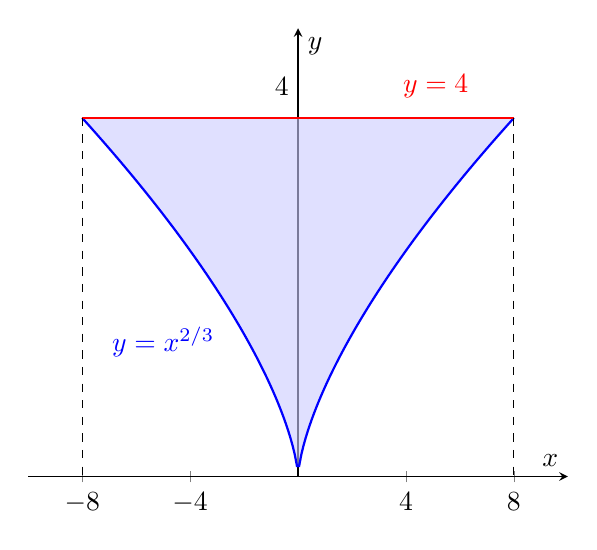
\begin{tikzpicture}
  \begin{axis}[
      xmin=-10, xmax=10,
      ymin=0, ymax=5,
      axis lines=middle,
      xlabel={$x$}, ylabel={$y$},
      clip=true,
      samples=200,
      ytick=\empty,
      scale=1,
      xtick distance=4,
    ]

    % Boundary curves
    \addplot[blue, thick, domain=-8:8] {abs(x)^(2/3)};
    \addplot[red, thick, domain=-8:8] {4};

    % Paths for shading
    \addplot[
      name path=lower,
      domain=-8:8,
      draw=none
    ] {abs(x)^(2/3)};

    \addplot[
      name path=upper,
      domain=-8:8,
      draw=none
    ] {4};

    % Shaded region
    \addplot[
      blue!20,
      opacity=0.6
    ] fill between [
      of=upper and lower
    ];
    \draw[dashed] (axis cs: -8,4) -- (axis cs: -8,0);
    \draw[dashed] (axis cs: 8,4) -- (axis cs: 8,0);

% Labels
\node at (axis cs:-5,1.5) [blue] {$y=x^{2/3}$};
\node at (axis cs:5.1,4.35) [red] {$y=4$};

% x-axis values
\node at (axis cs:-8,-0.35) {$-8$};
\node at (axis cs:8,-0.35) {$8$};

% y-axis value
\node at (axis cs:-0.6,4.35) {$4$};
\end{axis}
\end{tikzpicture}
\end{center}
\[\boxed{\int_0^4 \int_{-y^{3/2}}^{y^{3/2}} f(x, y)\,dx\,dy}\]

\item Using the suggested generalized polar coordinates $x=2r\cos\theta$ and $y=r\sin\theta$.
The Jacobian of this transformation is $J=2r.$
The boundary of the region D is the elliptic cylinder $x^{2}+4y^{2}=4$ which simplifies to $4r^{2}\cos^{2}\theta+4r^{2}\sin^{2}\theta=4\Rightarrow r=1$ Thus, $0\le r\le1$ and $0\le\theta\le2\pi$.
\begin{align*}
V &= \iint_{D}(x^{2}+y^{2})\,dA = \int_{0}^{2\pi}\int_{0}^{1}
     \left((2r\cos\theta)^{2}+(r\sin\theta)^{2}\right)
     (2r)\,dr\,d\theta \\
  &= \int_{0}^{2\pi}\int_{0}^{1}
     2r^{3}(4\cos^{2}\theta+\sin^{2}\theta)\,dr\,d\theta \\
  &= \left(\int_{0}^{1}2r^{3}\,dr\right)
     \left(\int_{0}^{2\pi}(4\cos^{2}\theta+\sin^{2}\theta)\,d\theta\right) \\
  &= \left[\frac{r^{4}}{2}\right]_{0}^{1}
     \cdot(4\pi+\pi)
   = \frac{1}{2}\cdot5\pi
   = \frac{5\pi}{2}
\end{align*}

$\boxed{\text{Answer: (C)}}$

\item For the paddle wheel to rotate counter-clockwise, the scalar curl ($z$-component of the curl) must be positive.
\[\text{curl}~\mathbf{F}\cdot\mathbf{k}=\frac{\partial}{\partial x}\left(-\frac{2}{x-2}\right)-\frac{\partial}{\partial y}(y^{2})=\frac{2}{(x-2)^{2}}-2y\]

Setting the curl greater than zero:
\[\frac{2}{(x-2)^{2}}-2y>0\Rightarrow2y<\frac{2}{(x-2)^{2}}\Rightarrow y<\frac{1}{(x-2)^{2}}\]

Since the question asks for the region above the x-axis, we also have $y>0$.

$\boxed{\text{Answer: (A)}}$

\item Let $u=x-y$ and $v=x+y$. The bounding lines become $u=0$, $u=2$, $v=0$, and $v=3$.

Solving for $x$ and $y$, we get $x=\frac{1}{2}(u+v)$ and $y=\frac{1}{2}(v-u)$.

The absolute value of the Jacobian determinant is $\frac{\partial(x,y)}{\partial(u,v)}=\frac{1}{2}$.

The integrand becomes $(x+y)e^{x^{2}-y^{2}}=ve^{uv}$.
\begin{align*}
\int_{0}^{3}\int_{0}^{2}ve^{uv}\left(\frac{1}{2}\right)du~dv
&=\frac{1}{2}\int_{0}^{3}[e^{uv}]_{u=0}^{u=2}dv
=\frac{1}{2}\int_{0}^{3}(e^{2v}-1)dv\\[1em]
&=\frac{1}{2}\left[\frac{1}{2}e^{2v}-v\right]_{0}^{3}
=\frac{1}{2}\left(\frac{1}{2}e^{6}-3-\left(\frac{1}{2}-0\right)\right)\\[1em]
&=\frac{1}{2}\left(\frac{1}{2}e^{6}-\frac{7}{2}\right)
=\frac{1}{4}(e^{6}-7)
\end{align*}

$\boxed{\text{Answer: (B)}}$

\item The field lines satisfy the differential equation $\frac{dy}{dx}=\frac{Q(x,y)}{P(x,y)}$.
\[
\frac{dy}{dx}=\frac{x}{y}\Rightarrow y~dy=x~dx
\]
Integrating both sides yields $\frac{1}{2}y^{2}=\frac{1}{2}x^{2}+K\Rightarrow x^{2}-y^{2}=C$

$\boxed{\text{Answer: (D)}}$

\item By the Divergence Theorem, the flux is $\iiint_{E}\text{div}\,\mathbf F~dV$.
\[\text{div}\,\mathbf F=3x^{2}+3y^{2}+3z^{2}=3\rho^{2}.\]
Using spherical coordinates for the unit sphere ($0\le\rho\le1,0\le\phi\le\pi,0\le\theta\le2\pi$).
\begin{align*}
\text{Flux}
&=\int_{0}^{2\pi}\int_{0}^{\pi}\int_{0}^{1}
(3\rho^{2})\rho^{2}\sin\phi~d\rho~d\phi~d\theta\\[1em]
&=3\left(\int_{0}^{2\pi}d\theta\right)
\left(\int_{0}^{\pi}\sin\phi~d\phi\right)
\left(\int_{0}^{1}\rho^{4}d\rho\right)
=3\cdot(2\pi)\cdot(2)\cdot\left(\frac{1}{5}\right)
=\frac{12\pi}{5}
\end{align*}

$\boxed{\text{Answer: (C)}}$

\item For $F_{1}=\langle-y,x,0\rangle$: $\text{div}\, \mathbf F_{1}=0+0+0=0$ (Solenoidal). $\text{curl}\,\mathbf F_{1}=\langle0,0,2\rangle\ne0$
For $\mathbf F_{2}=\langle x,y,z\rangle$: $\text{div}\,\mathbf F_{2}=1+1+1=3\ne0.$ $\text{curl}\,\mathbf F_{2}=\langle0,0,0\rangle$ (Irrotational).

$\boxed{\text{Answer: (C)}}$

\item We are looking for $\mathbf A=\langle0,\mathbf A_{2},\mathbf A_{3}\rangle$ such that $\nabla\times \mathbf A=\langle2y,z,0\rangle$.
\[
\nabla\times \mathbf A=\left\langle\frac{\partial \mathbf A_{3}}{\partial y}-\frac{\partial\mathbf A_{2}}{\partial z},-\frac{\partial \mathbf A_{3}}{\partial x},\frac{\partial \mathbf A_{2}}{\partial x}\right\rangle
\]

Equating components:

\begin{itemize}
    \item $\displaystyle-\frac{\partial\mathbf A_{3}}{\partial x}=z\Rightarrow \mathbf A_{3}=-xz+g(y,z)$
    
    \item $\displaystyle\frac{\partial\mathbf A_{2}}{\partial x}=0\Rightarrow \mathbf A_{2}=h(y,z)$
    
    \item $\displaystyle\frac{\partial\mathbf A_{3}}{\partial y}-\frac{\partial\mathbf A_{2}}{\partial z}=2y$
\end{itemize}

Substitute $\mathbf A_{3}$ and $\mathbf A_{2}$ into the third equation: $\frac{\partial g}{\partial y}-\frac{\partial h}{\partial z}=2y$.

There are infinitely many valid choices. A simple choice is to let $h(y,z)=0$ (so $\mathbf A_{2}=0$) Then
$\frac{\partial g}{\partial y}=2y\Rightarrow g(y,z)=y^{2}$ . This yields $\mathbf A_{3}=y^{2}-xz$.

Another valid choice is letting $g(y,z)=0$ (so $\mathbf A_{3}=-xz$). $-\frac{\partial h}{\partial z}=2y\Rightarrow h(y,z)=-2yz$.
This yields $\mathbf A_{2}=-2yz.$

Answer: (Using the first choice)
\[\boxed{\mathbf A(x,y,z)=\langle0,0,y^{2}-xz\rangle}\]
(Note: $\langle0,-2yz,-xz\rangle$ is also a correct valid pair).
Other valid answers are also welcome.
\end{enumerate}
\end{enumerate}

\end{document}